\scanpage{121}
\mspage{6}

I am going to give 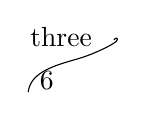
\begin{tikzpicture}[baseline=(oldcount.base),line cap=round,line join=round]
  \node[anchor=base west,inner sep=0pt] (oldcount) at (0,0) {\deleted{6}};
  \node[anchor=base west,inner sep=0pt] at (-.12,.54) {\inserted{three}};
  \draw[line width=.4pt] (-.14,-.03)
    .. controls (-.11,.20) and (.14,.29) .. (.46,.38)
    .. controls (.68,.44) and (.92,.56) .. (.98,.61)
    .. controls (1.01,.65) and (.98,.67) .. (.95,.63);
\end{tikzpicture} other presentations, where we eliminate not only the points near (say) the \deleted{$\unsure{R_\varphi|R_q}$} vertices of type 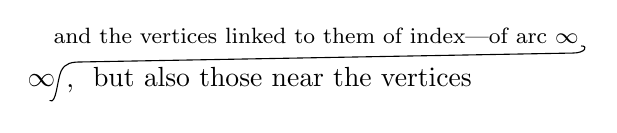
\begin{tikzpicture}[baseline=(continuation.base),line cap=round,line join=round]
  \node[anchor=base west,inner sep=0pt] at (-.55,0) {$\infty$};
  \node[anchor=base west,inner sep=0pt] at (-.06,-.01) {,};
  \node[anchor=base west,inner sep=0pt] (continuation) at (.28,0)
    {but also those near the vertices};
  \node[anchor=base west,inner sep=0pt,font=\footnotesize] (linkedinsert) at (-.22,.55)
    {\inserted{and the vertices linked to them \unsure{of index|of arc} $\infty$}};
  \draw[line width=.4pt] (-.26,-.18)
    .. controls (-.18,-.23) and (-.17,.07) .. (-.12,.19)
    .. controls (-.07,.30) and (.02,.31) .. (.15,.31)
    -- ([xshift=-.08cm,yshift=-.12cm]linkedinsert.south east)
    .. controls ([xshift=.08cm,yshift=-.12cm]linkedinsert.south east)
       and ([xshift=.12cm,yshift=-.03cm]linkedinsert.south east)
       .. ([xshift=.03cm,yshift=-.03cm]linkedinsert.south east);
\end{tikzpicture} (say) of type $1$, thus keeping only the vertices 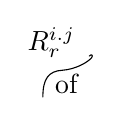
\begin{tikzpicture}[baseline=(typezero.base),line cap=round,line join=round]
  \node[anchor=base west,inner sep=0pt] (typezero) at (0,0) {of};
  \node[anchor=base west,inner sep=0pt] at (-.35,.55) {\inserted{$R_r^{i.j}$}};
  \draw[line width=.4pt] (-.15,-.04)
    .. controls (-.15,.19) and (-.08,.29) .. (.10,.30)
    .. controls (.25,.31) and (.41,.39) .. (.47,.46)
    .. controls (.49,.49) and (.47,.51) .. (.44,.48);
\end{tikzpicture} type $0$, i.e.
\[
(20)\qquad R_r^{0,1}\ \mathrel{\tikz[baseline=-.6ex,x=1em,y=1em,>=stealth]{\draw (.70,.70)--(.42,.42);\draw[->] (.29,.29)--(0,0);}}\qquad r\in\mathcal{R}
\]
\margin{$\boxed{R_r^{0,1}=R_{\sigma_\infty r}^{01}}$

redundancy relations for reference}
and we introduce the paths
\[
(21)\qquad\left\{\begin{aligned}
A_r^{0,1}&\overset{\text{def}}{=}(a_{\tau_0r}^\infty)^{-1}(\Lambda_r^{\prime1})^{-1}a_r^\infty:R_r^{0,1}\longrightarrow R_{\sigma_0(r)}^{0,1}\qquad(r\in\mathcal{R})\\
\Lambda_r^0&:R_r^{0,1}\longrightarrow R_{\sigma_1r}^{01}\qquad(r\in\mathcal{R})
\end{aligned}\right.
\]
\margin{plus the paths already known}
we have the redundancy relations
\[
(22)\qquad\boxed{\left\{\begin{aligned}
\Lambda_{\unsure{\sigma|r}}^0\Lambda_{\sigma_1(r)}^0&=1&&r\in\mathcal{R}\\
A_r^{0,1}A_{\sigma_0(r)}^{0,1}&=1&&r\in\mathcal{R}
\end{aligned}\right.}
\]
\figure{
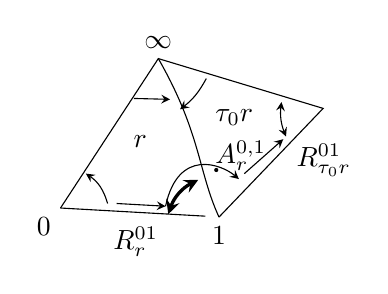
\begin{tikzpicture}[scale=1.15,>=stealth]
\coordinate (A) at (0,0);\coordinate (B) at (1.75,-0.10);\coordinate (C) at (1.08,1.65);\coordinate (D) at (2.90,1.10);
\draw (A)--(C)--(D)--(B);
% The lower outline stops just short of the vertex labelled 1 in the ink.
\draw (A)--(1.60,-0.09);
\draw (C)..controls(1.55,0.83)and(1.52,0.40)..(B);
\draw[->] (0.81,1.21)--(1.21,1.20);
\draw[->] (1.61,1.43) to[bend left=12] (1.32,1.09);
\draw[->] (0.52,0.05) to[bend right=20] (0.28,0.38);
\draw[->] (0.62,0.05)--(1.16,0.02);
\draw[very thick,<->] (1.19,-.068) to[bend left=22] (1.52,.31);
\draw[->] (1.16,0.02)..controls(1.30,0.67)and(1.78,0.48)..(1.97,0.32);
\draw[->] (2.03,0.38)--(2.46,0.76);
\draw[<->] (2.49,0.79) to[bend left=14] (2.44,1.17);
\fill (1.72,0.42) circle (0.023);
\node[below left] at (A) {$0$};\node[below] at (B) {$1$};\node[above] at (C) {$\infty$};
\node at (0.88,0.73) {$r$};\node at (1.92,1.00) {$\tau_0r$};\node at (1.99,0.58) {$A_r^{0,1}$};
\node[below] at (0.83,-0.10) {$R_r^{01}$};\node[right] at (2.50,0.53) {$R_{\tau_0r}^{01}$};
\end{tikzpicture}
}
and that is all: $\Pi_1(\widetilde{X}^{\substack{*\\*}*},\{R_r^{01}\}_{r\in\mathcal{R}})$ is \deleted{generated} \inserted{presented} by the vertices and arrows $(20)$ $(21)$, with only the redundancy relations $(20)$ $(22)$.

\uline{Filling holes} In each of the four cases considered, (in fact $10=1+3+3+3$ cases), the ``filling'' of a hole $R_{\unsure{\varphi s|s}}$ $(s\in S=S_0\amalg S_1\amalg S_\infty)$ is done in an essentially trivial way. In each of the four cases, one must, in terms of the chosen generating arrows, define \uline{the}

\mspage{120}
